\chapter{Introduction} 
\label{ch:introduction}

Mathematical and statistical models have long been used to describe or summarize observations in genetics and genomics.
Often without addressing the underlying biological mechanisms mutation, selection, and drift shaping DNA sequences, but as phenomelogical description.
However, as researchers learn more about the underlying processes and more genetic and genomic data is available, the mathematical descriptions allowing fo the extraction of information from this data have to keep up.
For example, after the unraveling of the degenerate genetic code by \citet{MatthaeiAndNirenberg1961,NirenbergAndMatthaei1961,Maxwell1962,LederAndNirenberg1964}, and many others, researchers noticed that synonymous codons are not found in uniform proportions \citep{fitch1976,grantham1980,ikemura1981,grantham1981,sharp1988}.
Models of codon usage, however, where long purely descriptive and heuristic \citep{ikemura1981,BennetzenAndHall1982,sharp1987,wright1990}.
Similarly, phylogenetic models have long been phenomelogical \citep{JukesAndCantor1969,Dayhoff1978,Kimura1980,felsenstein1981,Altschul1991}, describing the rate at which one state is transformed into another, without regards for the fundamental forces of evolution mutation, selection, and drift.
\citet{ZuckerkandlAndPauling1962} described the distance between hemoglobin proteins and proposed that the evolution of proteins is constant over time and between lineages before the genetic code was fully deciphered and were protein production was barely understood.
This dissertation is therefore focused on the application of mechanistic models rooted in first principles to protein coding sequences.

Mechanistic models are used throughout biology \citep{GoldmanAndYang1994,loreau1998,DavisAndPelsor2001,adf2007,McGill2007}.
By modeling the process underlying the observed data mechanistic models provide insights into the processes and estimates of parameters shaping the data \citep{Liberles2013}.
A wide variety of information is stored in protein and protein coding sequences, e.g. structure \citep{anfinsen1973}, mutation bias \citep{ShahAndGilchrist2011, gilchrist2015}, protein synthesis rate \citep{gilchrist2007,gilchrist2015}. 
Mechanistic models can be used extract these informations and to study the relative strength of mutation, selection, and genetic drift leading to the observed sequences.
Specifically, in this dissertation, mechanistic models lead to an understanding of the contributions of mutation, selection and drift on the evolution of observed sequences.

Protein production is the most costly metabolic process a cell performs \citep{buttgereit1995,warner1999,AkashiAndGojobori2002,lindqvist2018} yielding high selection to maximize the benefit of protein production.
Studying the cost/benefit ratio is therefore important to understand the evolution of protein coding sequences.
The interaction between cost and benefit cause for non-linear dynamics that are extremly difficult to model.
I therefore apply mechanistic models that either account for the cost or the benefit of protein production.


\section{Cost: Decomposing Codon Usage}

Mutation bias in codon usage is a reflection of the cellular environment while selection on codon usage allows us to make inferences about the cellular and external environment a genome and its genes are exposed to.
The relative strength of mutation and selection on individual genes varies, allowing us to separate the effects of mutation bias and selection, specifically selection against translation overhead cost \citep{gilchrist2007,ShahAndGilchrist2011,gilchrist2015}.
Genes with low protein synthesis rates are thought to be under weak selection and their codon usage is therefore dominated by mutation bias.
In contrast, genes with high protein synthesis rate are thought to be under strong selection and their codon usage is therefore dominated by selection.
However, mutation bias and selection can differ within the genome.
For example, strand specific mutation bias \citep{Lafay1999,Romero2000}, differences in the tRNA pool throughout life stages \citep{sagi2016}, or introgressionsand horizontal gene transfer \citep{medigue1991,lawrence1997} can produce or reflect of multiple genomic environments.
To provide researchers with a software tool, AnaCoDa \cite{landerer2018}, to address intra genomic variation in codon usage, chapter \ref{ch:anacoda} extends the mechanistic model ROC-SEMPPR \cite{gilchrist2015} to allow for a mixture distribution of mutation and selection parameters.
However, there is a significant difference to classical mixture approaches as ROC-SEMPPR not only estimates population specific parameters (mutation and selection) that are now modeled as mixture distributions but also a gene specific parameter (protein synthesis rate). 
Therefore, the protein synthesis rate has to be estimated for each population, providing additional insight into the adaptiveness of a gene to alternative genomic environments.

\begin{figure}[H]
     \centering
	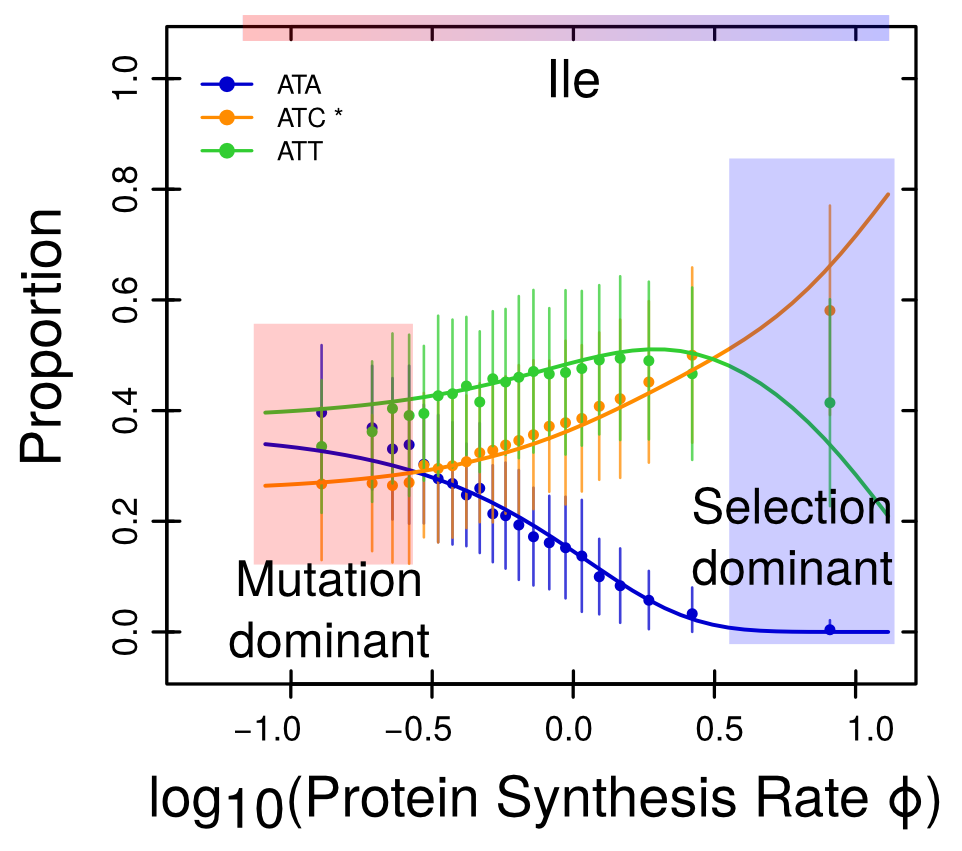
\includegraphics[width=0.6\textwidth]{ch1/expl_model}
	\caption{ROC-SEMPPER model behavior for Isoleucine.
	The proportion of each codon observed changes with protein synthesis rate.
	Mutation is dominant when protein synthesis rate is low, mutationally favored codons are observed with the highest frequency.
	With the increase of protein synthesis rate, the influence of selection increases until the system is dominated by selection.
	The selectively favored codon is observed with the highest frequency.}
	\label{fig:expl_model}
\end{figure}

In chapter \ref{ch:kluyveri}, I apply AnaCoDa to analyze the synonymous codon usage of the yeast \kluyveri which experienced a large scale introgression replacing the whole left arm of chromosome C \citep{friedrich2015}.
I studied the differences in the parameters describing codon usage between the endogenous \kluyveri genes and the introgressed exogenous genes.
Recognizing the differences in codon usage between the endogenous and exogenous genes allowed me to improve prediction of protein synthesis rate.
Applying a mechanistic models also allowed me to separate the effects of mutation and selection in the endogenous \kluyveri genes and the introgressed exogenous genes.
This information was used to determine a potential donor lineage in \gossypii, estimate a time since introgression, and estimate the genetic load the introgression introduced into the \kluyveri genome.

\section{Benefit: Selection on Amino acids}

In chapter \ref{ch:phylogeny}, I shifted my focus from the cost of protein synthesis to the functionality or benefit a protein produces.
For that matter I utilized a mechanistic phylogenetic model of stabilizing selection rooted in population genetics, SelAC \cite{beaulieu2018}.
I explore the selection on amino acids in the $\beta$-lactamase protein TEM.
 
\begin{figure}[H]
     \centering
	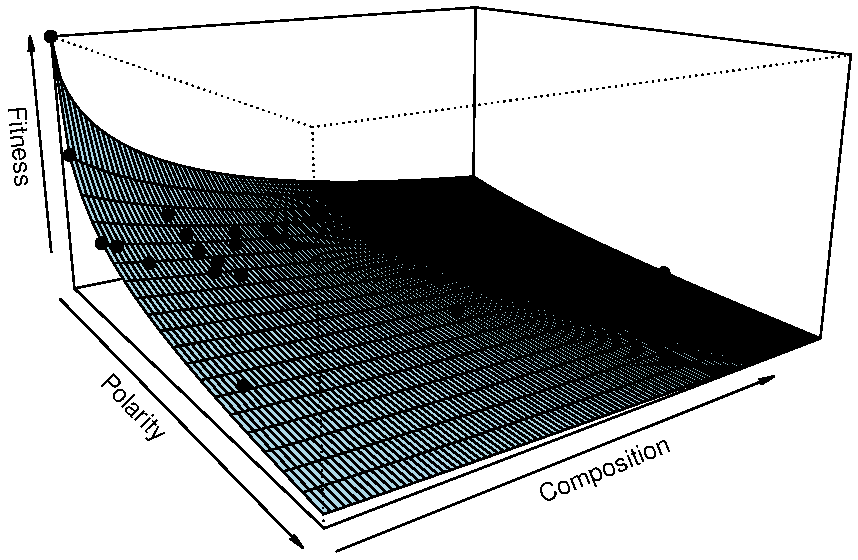
\includegraphics[width=0.7\textwidth]{ch1/decl_fitness2}
	\caption{Decline in fitness with distance in physicochemical space from the optimal amino acid. 
	Fitness decline of amino acids (black dots) relative to optimal amino acid (Alanine). Weighting of properties according to \citet{grantham1974}.}
	\label{fig:decl_fit}
\end{figure}

